\documentclass[12pt, xcolor={dvipsnames}, aspectratio = 169, sans,mathserif]{beamer}

\usepackage{fontspec}
\usepackage{fontawesome5}
\usepackage{mathrsfs}
\usepackage{amsmath, amssymb}
\usepackage{graphicx}
\usepackage{hyperref}
%\usepackage{physics}
\usepackage[absolute,overlay]{textpos}
\usepackage[font=tiny]{caption}
\usepackage[backend=bibtex, style=science]{biblatex}
\usepackage{standalone}
\usepackage{tikz}
\usetikzlibrary{shapes,arrows}


% Bib file
\addbibresource{NPrefs.bib}


% Custom Beamer theme
\usetheme{Hannover}

% Define the custom theme
\mode<presentation>


% Modify color scheme
\definecolor{nmsured}{RGB}{137,18,22} % NMSU colors
% \usecolortheme[named=nmsured]{structure}
\setbeamercolor{structure}{fg=nmsured} % Adjust structure color
\setbeamercolor{item}{fg=nmsured}
\setbeamercolor{frametitle}{bg=white, fg=nmsured}
\setbeamercolor{sidebar}{bg=nmsured!20}

\usefonttheme{serif}
\setbeamertemplate{footline}[frame number]
\setbeamertemplate{caption}[numbered]
\setbeamerfont{footnote}{size=\tiny}


% Some custom commands
\newenvironment{List}[2]
{\begin{textblock}{#1}#2
\begin{itemize}}
{\end{itemize}
\end{textblock}}

\newenvironment{Pic}[2]
{\begin{textblock}{#1}#2
\begin{figure}}
{\end{figure}
\end{textblock}}

\newcommand{\NPcite}[1]{{\tiny \footfullcite{#1}}}


\begin{document}

\title{Extraction of Drell-Yan Angular Coefficients using Neural Network-based Classifiers}
% \subtitle{Subtitle}
\author{Dinupa Nawarathne}
\institute{New Mexico State University \\
  Representing the E906/SeaQuest Collaboration \\
  FERMILAB-SLIDES-23-124-PPD
}

\date{New Perspectives Meeting - \today}

\titlegraphic{

\includegraphics[height=0.8cm]{imgs/Fermilab_logo.svg.png}

\includegraphics[height=0.8cm]{imgs/NMSU_logo.jpg}

\includegraphics[height=0.8cm]{imgs/SeaQuest.jpg}

\includegraphics[height=0.8cm]{imgs/DOE.png}
}

\begin{frame}
  \maketitle
\end{frame}

\begin{frame}
\frametitle{Table of Contents}
\tableofcontents
\end{frame}

\section{Methodology}
\subsection{Likelihood Ratio Test}

\begin{frame}
\frametitle{Likelihood Ratio Test}

\begin{List}{13.}{(2., 2.0)}

  \item The likelihood ratio test is a highly effective method for assessing the goodness of fit.

  \item Let $X_1, X_2, X_3, \ldots, X_n$ be a random sample from a distribution with a parameter $\theta$. Suppose that
  we have observed $X_1 = x_1, X_2 = x_2, \ldots, X_n = x_n$. We define the the likelihood function as the probability of
  the observed samples as a function of $\theta$;

  \begin{equation*}
  L(x_1, x_2, \ldots, x_n; \theta) = P(X_1=x_1, X_2=x_2, \ldots, X_n=x_n; \theta)
  \end{equation*}

  \item To decide between two simple hypotheses $H_0: \theta = \theta_0$
  and $H_1: \theta = \theta_1$, we define the likelihood ratio:

  \begin{equation*}
  \lambda(x_1, x_2, \ldots, x_n) = \frac{L(x_1, x_2, \ldots, x_n; \theta_0)}{L(x_1, x_2, \ldots, x_n; \theta_1)}
  \end{equation*}

\end{List}

\end{frame}

\begin{frame}
\frametitle{Likelihood Ratio Test}

\begin{List}{13.}{(2., 2.0)}

  \item To perform a likelihood ratio test, we choose a constant $c$. We reject $H_0$ if $\lambda < c$ and accept it if
  $\lambda \geq c$. The value of $c$ can be chosen based on the desired significance level $\alpha$.

  \item Neural networks excel at approximating non-linear functions, making them ideal for use as higher-dimensional
  likelihood functions.

  \item Our goal is to train the neural network to classify samples accurately. Specifically, we aim to classify samples
  $\omega_{0i} \in \Omega_0$ as $y = 0$ and $\omega_{1i} \in \Omega_1$ as $y = 1$, regardless of the parameter $\theta$.

  \item Subsequently, we can utilize the trained neural network to estimate any unknown parameter $\theta_{\text{unknown}}$ by employing
  the gradient descent algorithm.\NPcite{Andreassen:2019nnm}

\end{List}

\end{frame}

\subsection{Gaussian Example}

\begin{frame}
\frametitle{Gaussian Example}

\begin{List}{13.}{(2., 2.5)}

  \item Suppose we have a Gaussian distribution $\mathcal{N}(\mu_{\text{unknown}}, 1)$, where $\mu_{\text{unknown}}$ is
  the unknown parameter.

  \item Our training strategy is to train the neural network to classify samples drawn from two Gaussian distributions:
  $x_{0} \sim \mathcal{N}_{0}(0, 1)$ with the label $y = 0$, and $x_{1} \sim \mathcal{N}_{1}(\mu, 1)$ with the label $y = 1$,
  where $\mu$ can take any value within a specified range.

  \item We construct the neural network with three hidden layers, each layer consisting of 50 nodes.
  The layers are activated using the Rectified Linear Unit (ReLU), while the final layer is activated by the Sigmoid function.

  \item The neural network was trained for 200 epochs, employing early stopping with a patience of 10, to minimize the
  binary cross-entropy loss.

\end{List}

\end{frame}

\begin{frame}
\frametitle{Gaussian Example}

\begin{Pic}{6.0}{(2.0, 0.5)}
\scalebox{0.7}{
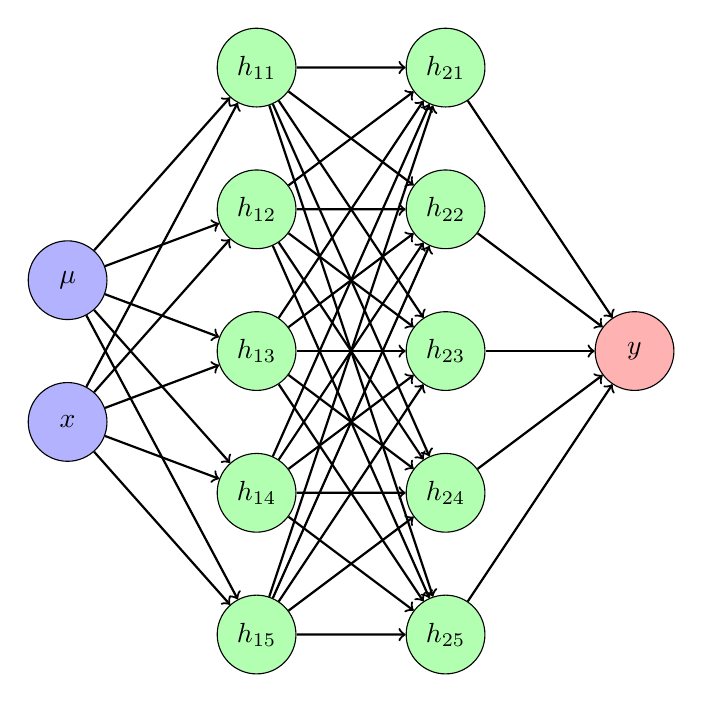
\begin{tikzpicture}[scale=1.2, every node/.style={draw, circle, minimum size=1cm}]
  % Input Layer
  \node[fill=blue!30] (input1) at (0,0.75) {$\mu$};
  \node[fill=blue!30] (input2) at (0,-0.75) {$x$};

  % Hidden Layers
  \node[fill=green!30] (hidden11) at (2, 3.0) {$h_{11}$};
  \node[fill=green!30] (hidden12) at (2, 1.5) {$h_{12}$};
  \node[fill=green!30] (hidden13) at (2, 0.0) {$h_{13}$};
  \node[fill=green!30] (hidden14) at (2,-1.5) {$h_{14}$};
  \node[fill=green!30] (hidden15) at (2,-3.0) {$h_{15}$};

  \node[fill=green!30] (hidden21) at (4, 3.0) {$h_{21}$};
  \node[fill=green!30] (hidden22) at (4, 1.5) {$h_{22}$};
  \node[fill=green!30] (hidden23) at (4, 0.0) {$h_{23}$};
  \node[fill=green!30] (hidden24) at (4,-1.5) {$h_{24}$};
  \node[fill=green!30] (hidden25) at (4,-3.0) {$h_{25}$};

  % Output Layer
  \node[fill=red!30] (output) at (6, 0.0) {$y$};

  % Arrows
  \draw[->, thick] (input1) -- (hidden11);
  \draw[->, thick] (input1) -- (hidden12);
  \draw[->, thick] (input1) -- (hidden13);
  \draw[->, thick] (input1) -- (hidden14);
  \draw[->, thick] (input1) -- (hidden15);
  \draw[->, thick] (input2) -- (hidden11);
  \draw[->, thick] (input2) -- (hidden12);
  \draw[->, thick] (input2) -- (hidden13);
  \draw[->, thick] (input2) -- (hidden14);
  \draw[->, thick] (input2) -- (hidden15);

  \draw[->, thick] (hidden11) -- (hidden21);
  \draw[->, thick] (hidden11) -- (hidden22);
  \draw[->, thick] (hidden11) -- (hidden23);
  \draw[->, thick] (hidden11) -- (hidden24);
  \draw[->, thick] (hidden11) -- (hidden25);

  \draw[->, thick] (hidden12) -- (hidden21);
  \draw[->, thick] (hidden12) -- (hidden22);
  \draw[->, thick] (hidden12) -- (hidden23);
  \draw[->, thick] (hidden12) -- (hidden24);
  \draw[->, thick] (hidden12) -- (hidden25);

  \draw[->, thick] (hidden13) -- (hidden21);
  \draw[->, thick] (hidden13) -- (hidden22);
  \draw[->, thick] (hidden13) -- (hidden23);
  \draw[->, thick] (hidden13) -- (hidden24);
  \draw[->, thick] (hidden13) -- (hidden25);

  \draw[->, thick] (hidden14) -- (hidden21);
  \draw[->, thick] (hidden14) -- (hidden22);
  \draw[->, thick] (hidden14) -- (hidden23);
  \draw[->, thick] (hidden14) -- (hidden24);
  \draw[->, thick] (hidden14) -- (hidden25);

  \draw[->, thick] (hidden15) -- (hidden21);
  \draw[->, thick] (hidden15) -- (hidden22);
  \draw[->, thick] (hidden15) -- (hidden23);
  \draw[->, thick] (hidden15) -- (hidden24);
  \draw[->, thick] (hidden15) -- (hidden25);

  \draw[->, thick] (hidden21) -- (output);
  \draw[->, thick] (hidden22) -- (output);
  \draw[->, thick] (hidden23) -- (output);
  \draw[->, thick] (hidden24) -- (output);
  \draw[->, thick] (hidden25) -- (output);
\end{tikzpicture}
}
\caption{Example of a neural network architecture: The input layer is depicted with blue nodes, the hidden layers are
represented by green nodes, and the output layer is indicated by a red node.}
\end{Pic}

\begin{Pic}{4.0}{(9.0, 1.5)}
\includegraphics[width=4.0cm]{imgs/ReLU.png}
\caption{ReLU activation function.}
\end{Pic}

\begin{Pic}{4.0}{(9.0, 8.0)}
\includegraphics[width=4.0cm]{imgs/Sigmoid.png}
\caption{Sigmoid activation function.}
\end{Pic}

\end{frame}

\begin{frame}
\frametitle{Gaussian Example}

\begin{Pic}{6.0}{(2.0, 0.5)}
\scalebox{0.7}{
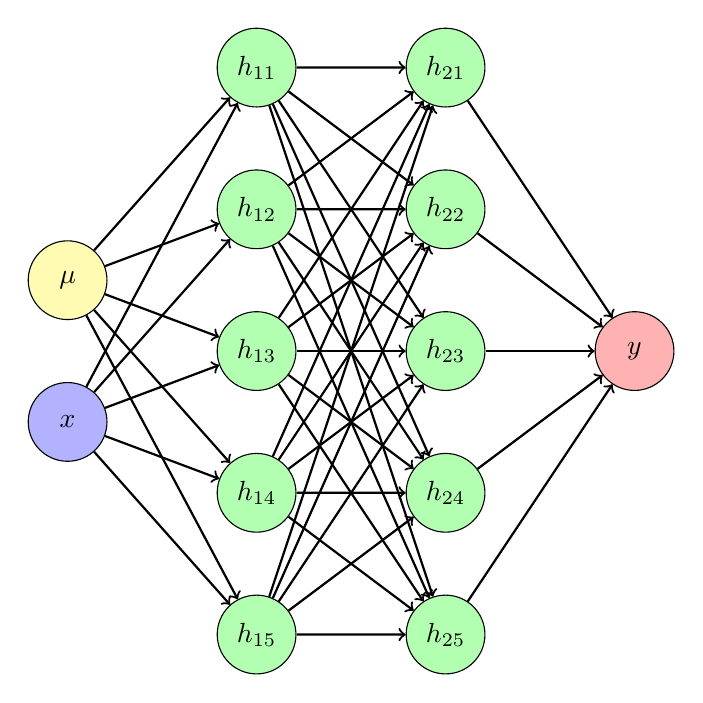
\begin{tikzpicture}[scale=1.2, every node/.style={draw, circle, minimum size=1cm}]
  % Input Layer
  \node[fill=yellow!30] (input1) at (0,0.75) {$\mu$};
  \node[fill=blue!30] (input2) at (0,-0.75) {$x$};

  % Hidden Layers
  \node[fill=green!30] (hidden11) at (2, 3.0) {$h_{11}$};
  \node[fill=green!30] (hidden12) at (2, 1.5) {$h_{12}$};
  \node[fill=green!30] (hidden13) at (2, 0.0) {$h_{13}$};
  \node[fill=green!30] (hidden14) at (2,-1.5) {$h_{14}$};
  \node[fill=green!30] (hidden15) at (2,-3.0) {$h_{15}$};

  \node[fill=green!30] (hidden21) at (4, 3.0) {$h_{21}$};
  \node[fill=green!30] (hidden22) at (4, 1.5) {$h_{22}$};
  \node[fill=green!30] (hidden23) at (4, 0.0) {$h_{23}$};
  \node[fill=green!30] (hidden24) at (4,-1.5) {$h_{24}$};
  \node[fill=green!30] (hidden25) at (4,-3.0) {$h_{25}$};

  % Output Layer
  \node[fill=red!30] (output) at (6, 0.0) {$y$};

  % Arrows
  \draw[->, thick] (input1) -- (hidden11);
  \draw[->, thick] (input1) -- (hidden12);
  \draw[->, thick] (input1) -- (hidden13);
  \draw[->, thick] (input1) -- (hidden14);
  \draw[->, thick] (input1) -- (hidden15);
  \draw[->, thick] (input2) -- (hidden11);
  \draw[->, thick] (input2) -- (hidden12);
  \draw[->, thick] (input2) -- (hidden13);
  \draw[->, thick] (input2) -- (hidden14);
  \draw[->, thick] (input2) -- (hidden15);

  \draw[->, thick] (hidden11) -- (hidden21);
  \draw[->, thick] (hidden11) -- (hidden22);
  \draw[->, thick] (hidden11) -- (hidden23);
  \draw[->, thick] (hidden11) -- (hidden24);
  \draw[->, thick] (hidden11) -- (hidden25);

  \draw[->, thick] (hidden12) -- (hidden21);
  \draw[->, thick] (hidden12) -- (hidden22);
  \draw[->, thick] (hidden12) -- (hidden23);
  \draw[->, thick] (hidden12) -- (hidden24);
  \draw[->, thick] (hidden12) -- (hidden25);

  \draw[->, thick] (hidden13) -- (hidden21);
  \draw[->, thick] (hidden13) -- (hidden22);
  \draw[->, thick] (hidden13) -- (hidden23);
  \draw[->, thick] (hidden13) -- (hidden24);
  \draw[->, thick] (hidden13) -- (hidden25);

  \draw[->, thick] (hidden14) -- (hidden21);
  \draw[->, thick] (hidden14) -- (hidden22);
  \draw[->, thick] (hidden14) -- (hidden23);
  \draw[->, thick] (hidden14) -- (hidden24);
  \draw[->, thick] (hidden14) -- (hidden25);

  \draw[->, thick] (hidden15) -- (hidden21);
  \draw[->, thick] (hidden15) -- (hidden22);
  \draw[->, thick] (hidden15) -- (hidden23);
  \draw[->, thick] (hidden15) -- (hidden24);
  \draw[->, thick] (hidden15) -- (hidden25);

  \draw[->, thick] (hidden21) -- (output);
  \draw[->, thick] (hidden22) -- (output);
  \draw[->, thick] (hidden23) -- (output);
  \draw[->, thick] (hidden24) -- (output);
  \draw[->, thick] (hidden25) -- (output);
\end{tikzpicture}
}
\caption{In the fitting step, the only trainable parameter is the yellow node representing $\mu$.}
\end{Pic}

\begin{List}{7.5}{(8.0, 3.0)}

  \item To perform the fitting algorithm, we fix the weights and biases of the trained neural network.
  Then, we optimize the $\mu$ parameter by using the gradient descent algorithm to find the optimal value $\mu_{\text{opt}}$.

\end{List}

\end{frame}

\begin{frame}
\frametitle{Gaussian Example}

\begin{Pic}{6.5}{(2.0, 1.0)}
\includegraphics[width=6.5cm]{imgs/opt_1D.png}
\caption{We tested the algorithm with $\mu_{\text{unknown}} = 1.3$. As depicted in the plot, the optimal value for $\mu$
converges to the correct value as the epochs progress.}
\end{Pic}

\begin{Pic}{6.5}{(9.0, 1.0)}
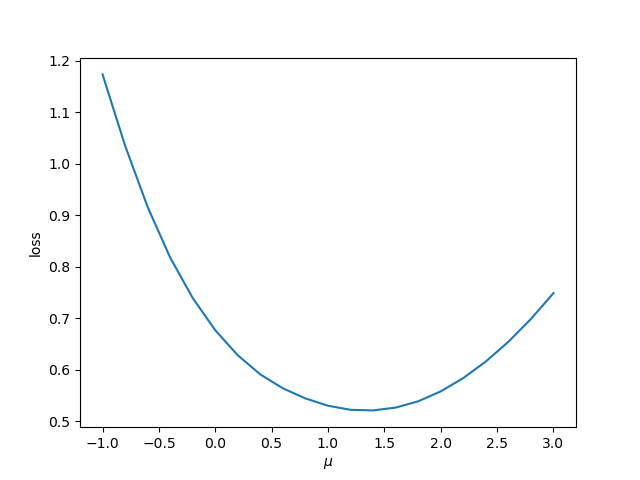
\includegraphics[width=6.5cm]{imgs/loss1D.png}
\caption{The loss reaches its minimum value at the optimal value of $\mu$.}
\end{Pic}

\end{frame}

\section{Drell-Yan Angular Coefficients}
\subsection{Drell-Yan Cross Section}

\begin{frame}
\frametitle{Drell-Yan Cross Section}

\begin{Pic}{5.0}{(2.0, 0.5)}
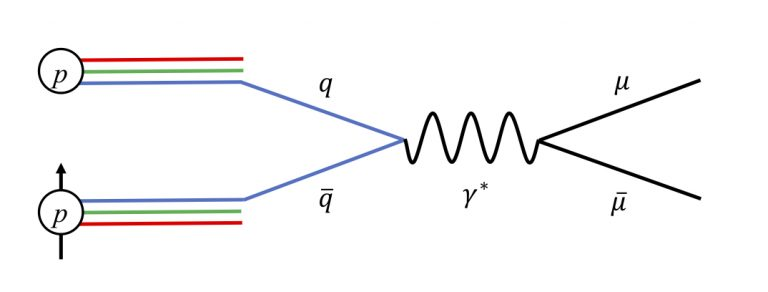
\includegraphics[width=5.0cm]{imgs/Drell-Yan.png}
\caption{Drell-Yan process.}
\end{Pic}

\begin{textblock}{8.0}(7.5, 2.0)
\begin{equation*}
\frac{d\sigma}{d\Omega} \propto 1 + \lambda cos^{2}\theta + \mu sin2\theta cos\phi + \frac{\nu}{2} sin^{2}\theta cos2\phi
\end{equation*}
\end{textblock}

\begin{List}{13.0}{(2.0, 7.0)}

  \item In the ``naive" Drell-Yan model, where we ignore the transverse momentum of the quark and assume no gluon emission,
  we have $\lambda = 1$, $\mu = \nu = 0$.

  \item Measuring the $\cos 2\phi$ angular dependence can be used to extract the Boer-Mulders (BM) function.

  \item BM function describes the transverse-polarization asymmetry of quarks within an unpolarized hadron and results
  from the coupling between the transverse momentum and transverse spin of the quarks inside the hadron.

\end{List}

\end{frame}


\subsection{FermiLab E906/SeaQuest Experiment}

\begin{frame}
\frametitle{FermiLab E906/SeaQuest Experiment}

\begin{Pic}{13.}{(2.0, 1.0)}
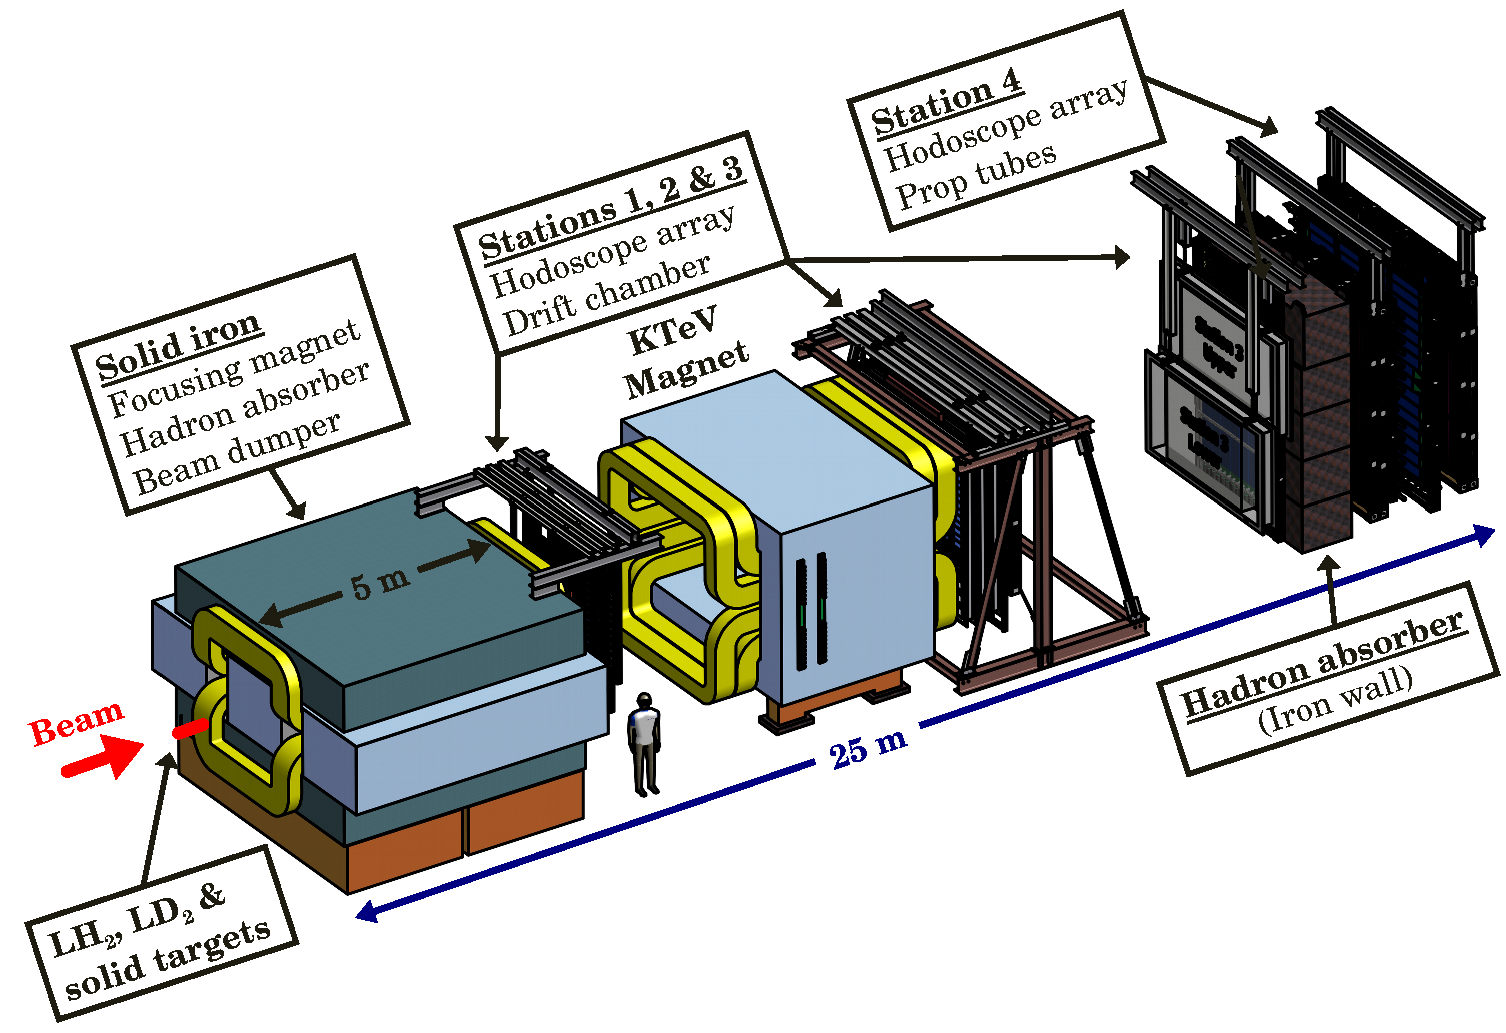
\includegraphics[width=9.0cm]{imgs/spectrometer.png}
\caption{FermiLab E906/SeaQuest spectrometer.}
\end{Pic}

\end{frame}

\subsection{Applying the Fitting Algorithm to E906 MC Data}

\begin{frame}
\frametitle{Applying the Fitting Algorithm to E906 MC Data}

\begin{List}{13.}{(2., 3.)}

  \item We generated the Monte Carlo (MC) data using the PYTHIA generator. The generated events were then passed through
  the E906 detector simulation (using GEANT4) to obtain the reconstructed detector information. As input features for the neural network,
  we use the mass, $p_{T}$, $x_{F}$, $\phi$, and $\cos\theta$.

  \item We sample the values of $\lambda$, $\mu$ and $\nu$ uniformly  from the ranges of (0.5, 1.5), (−0.5, 0.5), and
  (−0.5, 0.5), respectively.\NPcite{NuSea:2006gvb}

  \item The neural network consists of five hidden linear layers, each containing 64 nodes. The ReLU function is used
  to activate the hidden layers, along with batch normalization layers. The final output is passed through a Sigmoid activation function.

\end{List}

\end{frame}

\begin{frame}
\frametitle{Applying the Fitting Algorithm to E906 MC Data}

\begin{List}{13.}{(2., 3.)}

  \item The neural network was trained for 200 epochs, employing early stopping with a patience of 20, to minimize the
  binary cross-entropy loss.

  \item We conducted a sanity check using four different combinations of $\lambda$, $\mu$, and $\nu$. The fitted values
  are presented in table \ref{tabel:1}.

  \item In the five test samples, we were able to extract the injected parameters within a $\pm$1.5 standard deviation ($\sigma$) interval.

\end{List}

\end{frame}

\begin{frame}
\frametitle{Applying the Fitting Algorithm to E906 MC Data}

\begin{center}
\begin{table}
\begin{tabular}{ |c| c| c| c| }
\hline
Combination & Coefficient & Injected & Fitted \\
\hline
1           & $\lambda$   & 0.84      & 0.876 $\pm$ 0.208 \\
            & $\mu$       & 0.26      & 0.234 $\pm$ 0.054 \\
            & $\nu$       & -0.34      & -0.299 $\pm$ 0.052 \\
\hline
2           & $\lambda$   & 1.33      & 1.134 $\pm$ 0.151 \\
            & $\mu$       & 0.17      & 0.146 $\pm$ 0.050 \\
            & $\nu$       & -0.34      & -0.281 $\pm$ 0.043 \\
\hline
3           & $\lambda$   & 1.12      & 1.242 $\pm$ 0.181 \\
            & $\mu$       & -0.27      & -0.211 $\pm$ 0.088 \\
            & $\nu$       & -0.24      & -0.236 $\pm$ 0.071 \\
\hline
4           & $\lambda$   & 0.62      & 0.888 $\pm$ 0.282 \\
            & $\mu$       & -0.32      & -0.232 $\pm$ 0.091 \\
            & $\nu$       & 0.18      & 0.147 $\pm$ 0.055 \\
\hline

\end{tabular}
  \caption{Table showing the fitted values of $\lambda$, $\mu$, and $\nu$ using the gradient descent algorithm.}
  \label{tabel:1}
\end{table}
\end{center}

\end{frame}

\section{Summary}

\begin{frame}
\frametitle{Summary}

\begin{List}{13.}{(2., 1.5)}

  \item Neural networks can be used as multi-dimensional likelihood functions, and we can utilize likelihood ratio test
  to extract the optimal parameters for the Drell-Yan angular distribution.

  \item Measuring the $\cos2\phi$ angular dependence with higher accuracy is important for extracting the Boer-Mulders
  (BM) functions.

  \item BM function describes the transverse-polarization asymmetry of quarks within an unpolarized hadron and results
  from the coupling between the transverse momentum and transverse spin of the quarks inside the hadron. This function
  serves as a useful tool for unraveling the structure of hadrons.

  \item Our plan is to use this high-dimensional fitting algorithm to extract the Drell-Yan angular coefficients from the
  E906/SeaQuest data with higher accuracy.

  \item Acknowledgement: This work was funded by the DOE Office of Science, Medium-Energy Nuclear Physics Program.

\end{List}

\end{frame}

\begin{frame}{Neural Network}

\begin{List}{13.}{(2., 2.)}

  \item Think of a neural network as a network of interconnected nodes, called neurons, organized in layers. The input
  layer receives information, such as numerical data, images, or text. This information is then passed through the network,
  layer by layer, where each neuron performs a simple calculation based on its input and a set of weights.

  \item During training, the neural network adjusts these weights based on the provided input and the desired output.
  It learns by continuously comparing its predictions to the actual results and updating the weights accordingly, aiming
  to minimize the difference between them. This process, known as backpropagation, allows the network to learn and improve
  its performance over time.

\end{List}

\end{frame}

\begin{frame}{Neural Network}

\begin{List}{13.}{(2., 2.)}

  \item Once trained, the neural network can make predictions or classify new, unseen data based on the patterns it has learned.
  It can handle a wide range of tasks, including image and speech recognition, natural language processing, and predictive modeling.

  \item Learning Rate: The learning rate is a hyperparameter that determines how quickly a neural network adapts its weights during
  training. It controls the step size taken in the direction of minimizing the loss function. A higher learning rate can lead
  to faster convergence, but it may also cause overshooting and instability. On the other hand, a lower learning rate can
  ensure more stable updates, but it may slow down the convergence. Finding an appropriate learning rate is crucial for
  effective training.

\end{List}

\end{frame}

\begin{frame}{Neural Network}

\begin{List}{13.}{(2., 2.)}

  \item Early Patience (Early Stopping): Early patience, also known as early stopping, is a technique used to prevent overfitting
  and improve generalization in a neural network. During training, the model's performance is monitored on a validation set. If the
  validation loss stops improving or starts to worsen after a certain number of epochs, early patience is applied. It involves
  stopping the training process early and using the model with the best validation performance as the final model. Early patience
  helps to prevent the model from overfitting to the training data and ensures it generalizes well to unseen data.

\end{List}

\end{frame}

\begin{frame}{Neural Network}

\begin{List}{13.}{(2., 2.)}

  \item The binary cross entropy loss is calculated as follows;

  \begin{equation*}
  \mathcal{L}(y, \hat{y}) = - (y* log(\hat{y}) + (1-y)* log(1 - \hat{y}))
  \end{equation*}

  where $y$ represents the true binary label (either 0 or 1) of the training example. $\hat{y}$ represents the predicted probability
  of the positive class (typically obtained by passing the input through a sigmoid activation function).

\end{List}

\end{frame}

\end{document}
